\documentclass[slovak]{article}
\usepackage[dvips]{graphicx}        % to include images
\usepackage{pslatex}	    % to use PostScript fonts
\usepackage[T1]{fontenc}
\usepackage[utf8]{inputenc}
\usepackage{pslatex}

\usepackage{tabularx} % tabulky na celu sirku strany
\usepackage{graphicx} %graphics files inclusion
\usepackage{multirow}
\usepackage{mathtools}
\usepackage{listings}
\usepackage{pdfpages}

\hyphenation{pa-ra-le-li-zu-je-me}
\hyphenation{do-sia-hli}

\begin{document}

\title{Semestrálna práca MI-PAP 2013/2014: \\[5mm] Násobenie matíc}
\author{Martin Klepáč \\[2mm]Pavol Kušlita}
\date{\today}

\maketitle

\section{Definícia problému}

Našou úlohou bolo vytvoriť program, ktorý implementuje násobenie matíc formou ako klasického algoritmu, tak aj s použitím Strassenovho algoritmu. 

\section{Formát vstupu, výstupu}

Formálne, vstup vyjadríme pomocou

\begin{itemize}

\item \emph{A, B} = vstupné matice

\item \emph{Ax, Ay, Bx, By} = dimenzie vstupných matíc A, B

\end{itemize}

Výstupom algoritmu je matica \emph{C} s dimenziami \emph{Ax}, \emph{By} za podmienky, že \emph{Ay} = \emph{Bx}. V opačnom prípade nie je možno vykonať násobenie vstupných matíc.


\section{Implementácia sekvenčného riešenia}

Sekvenčný algoritmu pozostáva z trojice cyklov, ktoré prechádzajú matice \emph{A}, \emph{B} v nasledovnom poradí:

\begin{enumerate}

\item riadok matice \emph{A}

\item stĺpec matice \emph{B}

\item stĺpec matice \emph{A}, ktorý zároveň predstavuje riadok matice \emph{B}

\end{enumerate}

Vo najvnútornejšom cykle sa potom vykoná samotný výpočet popísaný pseudokódom nižšie:

\begin{verbatim}
C[i][j] += A[i][k] * B[k][j];
\end{verbatim}

Zložitosť takéhoto výpočtu je potom intuitívne $\mathcal{O}$($n^3$). Zároveň tento triviálny algoritmus nevyužíva možnosti cache pamäte.

Vylepšenie tohto triviálneho algoritmu spočíva v použití techniky loop-tiling. Výsledkom je zdvojnásobenie celkového počtu cyklov na 6, pričom miesto sekvenčného posunu indexov \emph{i} až \emph{k} posúvame indexy v našom prípade o 100, aby sme následne iterovali pomocnými indexami \emph{ii}, \emph{jj} respktíve \emph{kk} medzi 0-99, 100-199 a tak ďalej. Výsledkom je rovnaké množstvo vykonanej práce pri efektívnejšom využití cache pamäte. Pseudokód popisujúci techniku loop tiling-u:

\begin{verbatim}
for i in 0..Ax
 for j in 0..By
  for k in 0..Ay
   for ii in i..i+100 
    for jj in j..j+100
     for kk in k..k+100
      C[ii][jj] += A[ii][kk] * B[kk][jj];
\end{verbatim}

Strassenov algoritmus je asymptoticky rýchlejší než štandardný multiplikatívny algoritmus. Jeho asymptotická zložitosť je $\mathcal{O}$($n^{2.8074}$). Jedna sa o rekurzivný algoritmus, ktorý maticu \emph{A} a \emph{B} rozdeli na podmatice \emph{A_{11}},\emph{A_{12}},\emph{A_{21}},\emph{A_{22}} a podobne aj maticu \emph{B}. 

A =
 \begin{pmatrix}
  A_{11} & A_{12} \\
  A_{21} & A_{22} \\
 \end{pmatrix}

Následne do pomocných matíc M1 až M7, uloží čiastočné výsledky násobenia. V tomto kroku dochádza k zrýchleniu voči klasickému násobeniu, kedže dochádza iba k siedmym násobeniam. Pri týchto siedmych násobeniach opäť využívame Strassenov algoritmus až do určitej hranice, pri ktorej je už efektívnejšie používať klasický spôsob. Táto hranica závisí od implementácie a od hardvéru. V našom prípade bola empirický stanovená na hodnotu 64. Na konci algoritmu sa medzivýsledky v pomocných maticiach M1 až M7 spoja a vytvoria matice C1, C2, C3, C4, ktoré spolu vytvárajú výslednú maticu C.

\section{Implementácia paralelného riešenia pomocou OpenMP}

Prostredie OpenMP sa ukázalo byť veľmi jednoduché na implementáciu triviálneho algoritmu s použitím viacerých vlákien. Vzhľadom na to, že objem práce v najvnútornejšom cykle je rovnaký pre všetky vlákna, použili sme statické rozdelenie záťaže priamo v prostredí OpenMP definované kľúčovým slovom \emph{static}. Aby sme v prípade menších vstupných matíc v kombinácii s väčším počtom vlákien zamedzili plytvaniu prostriedkov, miesto jedného cyklu paralelizujeme dvojicu vonkajších cyklov s pomocou kľúčového slova \emph{collapse}.

Kód definujúci paralelizáciu ako triviálneho algoritmu, tak aj algoritmu s použitím loop tiling-u vyzerá nasledovne:

\begin{verbatim}
#pragma omp parallel for collapse (2) default(shared) private(i,j,k)
schedule(static)
\end{verbatim}

<TO DO - Strassenov algoritmus paralelne>

\section{Merania}

Pre potreby merania na serveri star.fit.cvut.cz sme vygenerovali trojicu pseudonáhodných štvorcových matíc o veľkosti 1024, 2048 a 4096. Program samozrejme dokáže spracovať aj iné ako štvorcové matice, ale pre férové porovnanie Strassenovho algoritmu s ostatnými riešeniami, používame práve štvorcové matice o veľkosti  $2^n$ - naša implementácia Strassena automaticky dopĺňa vstupné matice na najbližšiu vyššiu takúto veľkosť.

Namerané hodnoty sú uvedené v tabuľke \ref{tab1} pre dané vstupné matice, počet vlákien 1, 2, 4, 6, 8, 12, 24 pre všetky hore popísané implementácie. Výsledné hodnoty predstavujú aritmetický priemer trojice meraní.

	\begin{table}\centering
		\begin{tabularx}{\textwidth}{|X|X|X|X|X|X|X|X|X|X|}
			\hline                        
			& \multicolumn{3}{|c|}{\textbf{1024x1024}} & \multicolumn{3}{|c|}{\textbf{2048x2048}} & \multicolumn{3}{|c|}{\textbf{4096x4096}} \\ \hline
			& \textbf{CL} & \textbf{LT} & \textbf{ST} & \textbf{CL} & \textbf{LT} & \textbf{ST} & \textbf{CL} & \textbf{LT} & \textbf{ST} \\ \hline
			\textbf{-n 1} & 11.33	& 10.02 & 4.85  & 125.20 & 79.60 & 34.15 & 1347.2 & 651.67 & 239.81\\ \hline
			\textbf{-n 2} & 5.84	& 5.47 &  2.82  & 56.44 & 41.22 & 19.82  & 565.86 & 327.14 & 138.82\\ \hline
			\textbf{-n 4} & 2.93	& 2.82 &  1.49  & 30.03 & 20.79 & 10.21  & 302.63 & 163.87 & 70.66\\ \hline
			\textbf{-n 6} & 1.96	& 1.94 &  1.10  & 20.59 & 13.96 & 7.35   & 203.99 & 109.19 & 52.04\\ \hline
			\textbf{-n 8} & 1.48	& 1.46 &  0.85  & 16.33 & 10.57 & 5.80   & 158.66 & 81.65 & 39.93\\ \hline
			\textbf{-n 12} & 0.98	& 1.07 &  0.60  & 10.74 & 7.05 & 3.96    & 114.60 & 56.16 & 27.91\\ \hline
			\textbf{-n 24} & 0.92	& 0.81 &  0.50  & 8.40 & 5.87 & 3.14     & 83.37 & 50.18 & 19.71\\ \hline
		\end{tabularx}
	\caption{Trvanie behu v sekundách na OpenMP (CL = classic, LT = loop-tiling, ST = Strassen)}
	\label{tab1}
	\end{table}

Nasledovné grafy znázorňujú ako paralelný čas, tak aj paralelnú cenu pre všetky tri vstupy pre variabilný počet vlákien.

\begin{figure}\centering
	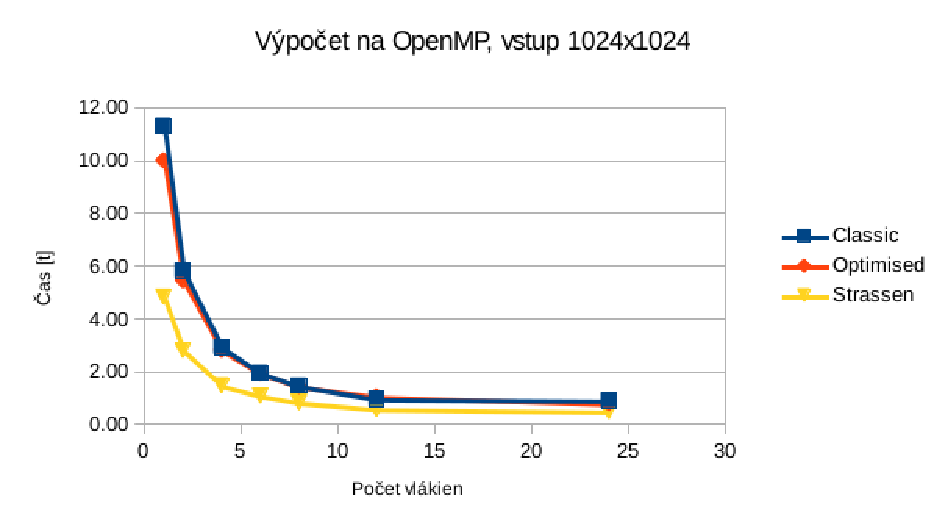
\includegraphics[scale=1]{./images/1024_rychlost.pdf}
	\label{gr:graf1}
\end{figure}

\begin{figure}\centering
	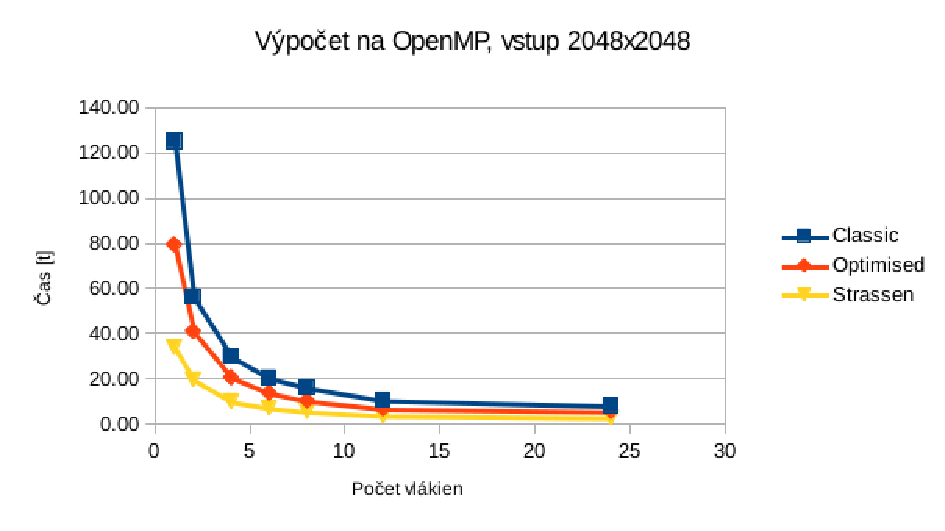
\includegraphics[scale=1]{./images/2048_rychlost.pdf}
	\label{gr:graf2}
\end{figure}  

\begin{figure}\centering
	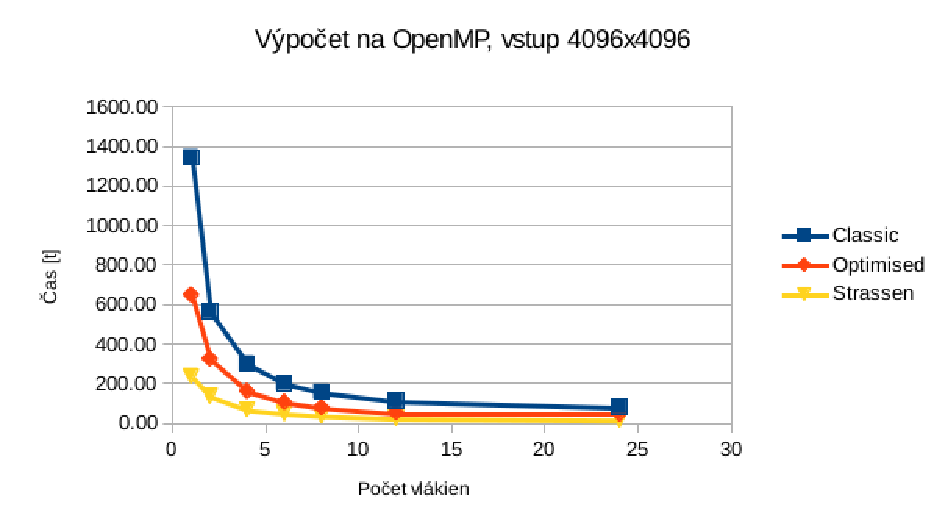
\includegraphics[scale=1]{./images/4096_rychlost.pdf}
	\label{gr:graf3}
\end{figure}  

\begin{figure}\centering
	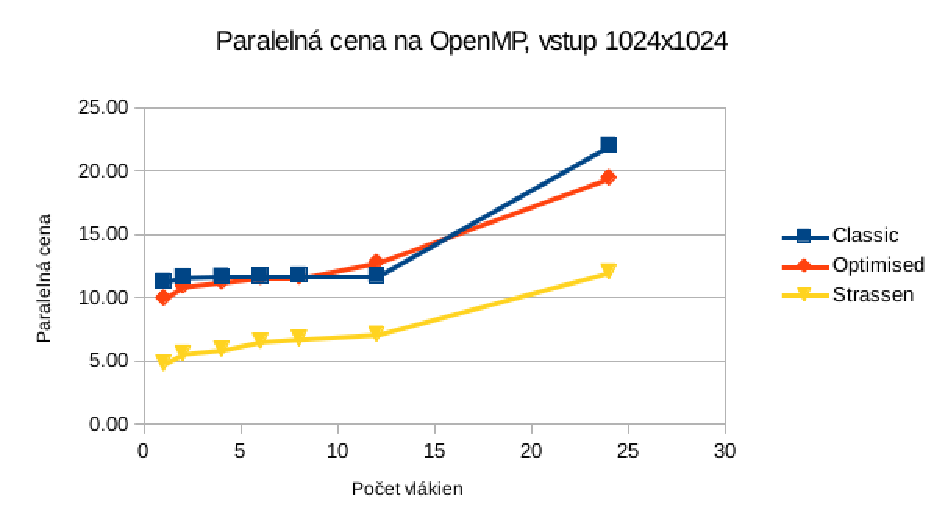
\includegraphics[scale=1]{./images/1024_cena.pdf}
	\label{gr:graf4}
\end{figure}  

\begin{figure}\centering
	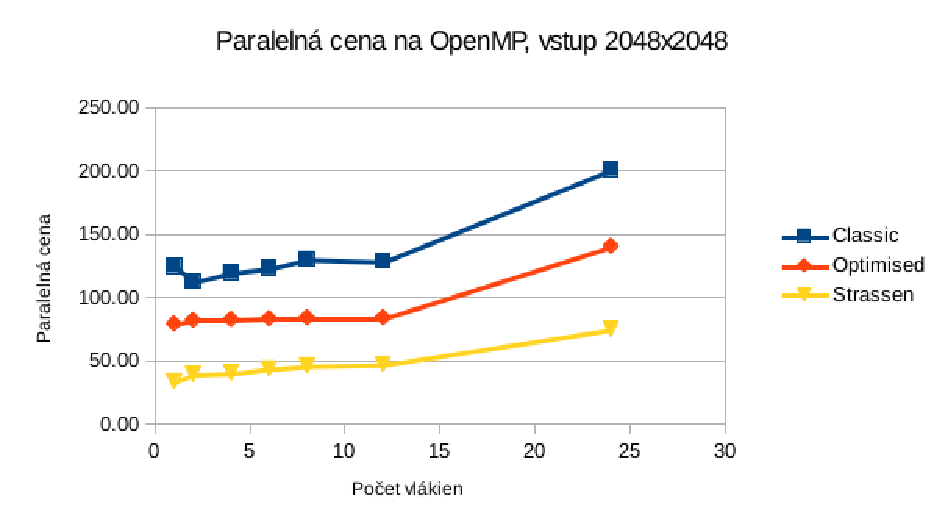
\includegraphics[scale=1]{./images/2048_cena.pdf}
	\label{gr:graf5}
\end{figure}  

\begin{figure}\centering
	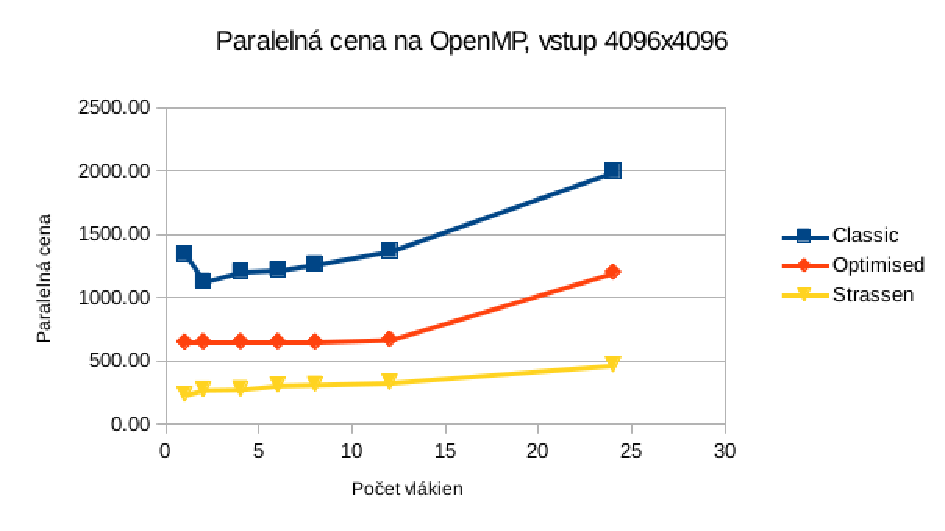
\includegraphics[scale=1]{./images/4096_cena.pdf}
	\label{gr:graf6}
\end{figure}  

Ako môžeme vidieť, pre takmer všetky vlákna (výnimkou je 24 vlákien) a všetky implementácie sme dosiahli približne lineárne zrýchlenie, a teda konštantnú paralelnú cenu. Zvýšenie paralelnej ceny pre 24 vlákien spočíva v tom, že nami použitý hardvér nemal k dispozícii 24 fyzických procesorov, a teda zákonite došlo k prepínaniu kontextu v rámci jedného fyzického procesora. V porovnaní s predmetom BI-PPR, na ktorom sme pracovali s distribuovanou pamätťou, nedošlo k superlineárnemu zrýchleniu. 

Ak by sme porovnávali jednotlivé implementácie medzi sebou, klasický a optimalizovaný algoritmus majú rovnakú asymptotickú zložitosť. Napriek tomu dosahuje optimalizovaná verzia zrýchlenie približne v rozsahu 10 až 50 percent v závislosti od veľkosti vstupu (čím väčší vstup, tým väčšie zrýchlenie). Strassenov algoritmus, ktorého zložitosť je $\mathcal{O}$($n^{2.8074}$), dosahuje v porovnaní s optimalizovanou variantou zrýchlenie približne o 50 percent.

\end{document}
